\hypertarget{stm32f4xx__hal__i2c__ex_8c}{}\section{Dokumentacja pliku S\+T\+M/\+W\+D\+S\+\_\+\+Kosc\+\_\+\+Linux/\+Drivers/\+S\+T\+M32\+F4xx\+\_\+\+H\+A\+L\+\_\+\+Driver/\+Src/stm32f4xx\+\_\+hal\+\_\+i2c\+\_\+ex.c}
\label{stm32f4xx__hal__i2c__ex_8c}\index{S\+T\+M/\+W\+D\+S\+\_\+\+Kosc\+\_\+\+Linux/\+Drivers/\+S\+T\+M32\+F4xx\+\_\+\+H\+A\+L\+\_\+\+Driver/\+Src/stm32f4xx\+\_\+hal\+\_\+i2c\+\_\+ex.\+c@{S\+T\+M/\+W\+D\+S\+\_\+\+Kosc\+\_\+\+Linux/\+Drivers/\+S\+T\+M32\+F4xx\+\_\+\+H\+A\+L\+\_\+\+Driver/\+Src/stm32f4xx\+\_\+hal\+\_\+i2c\+\_\+ex.\+c}}


I2C Extension H\+AL module driver. This file provides firmware functions to manage the following functionalities of I2C extension peripheral\+:  


{\ttfamily \#include \char`\"{}stm32f4xx\+\_\+hal.\+h\char`\"{}}\newline
Wykres zależności załączania dla stm32f4xx\+\_\+hal\+\_\+i2c\+\_\+ex.\+c\+:\nopagebreak
\begin{figure}[H]
\begin{center}
\leavevmode
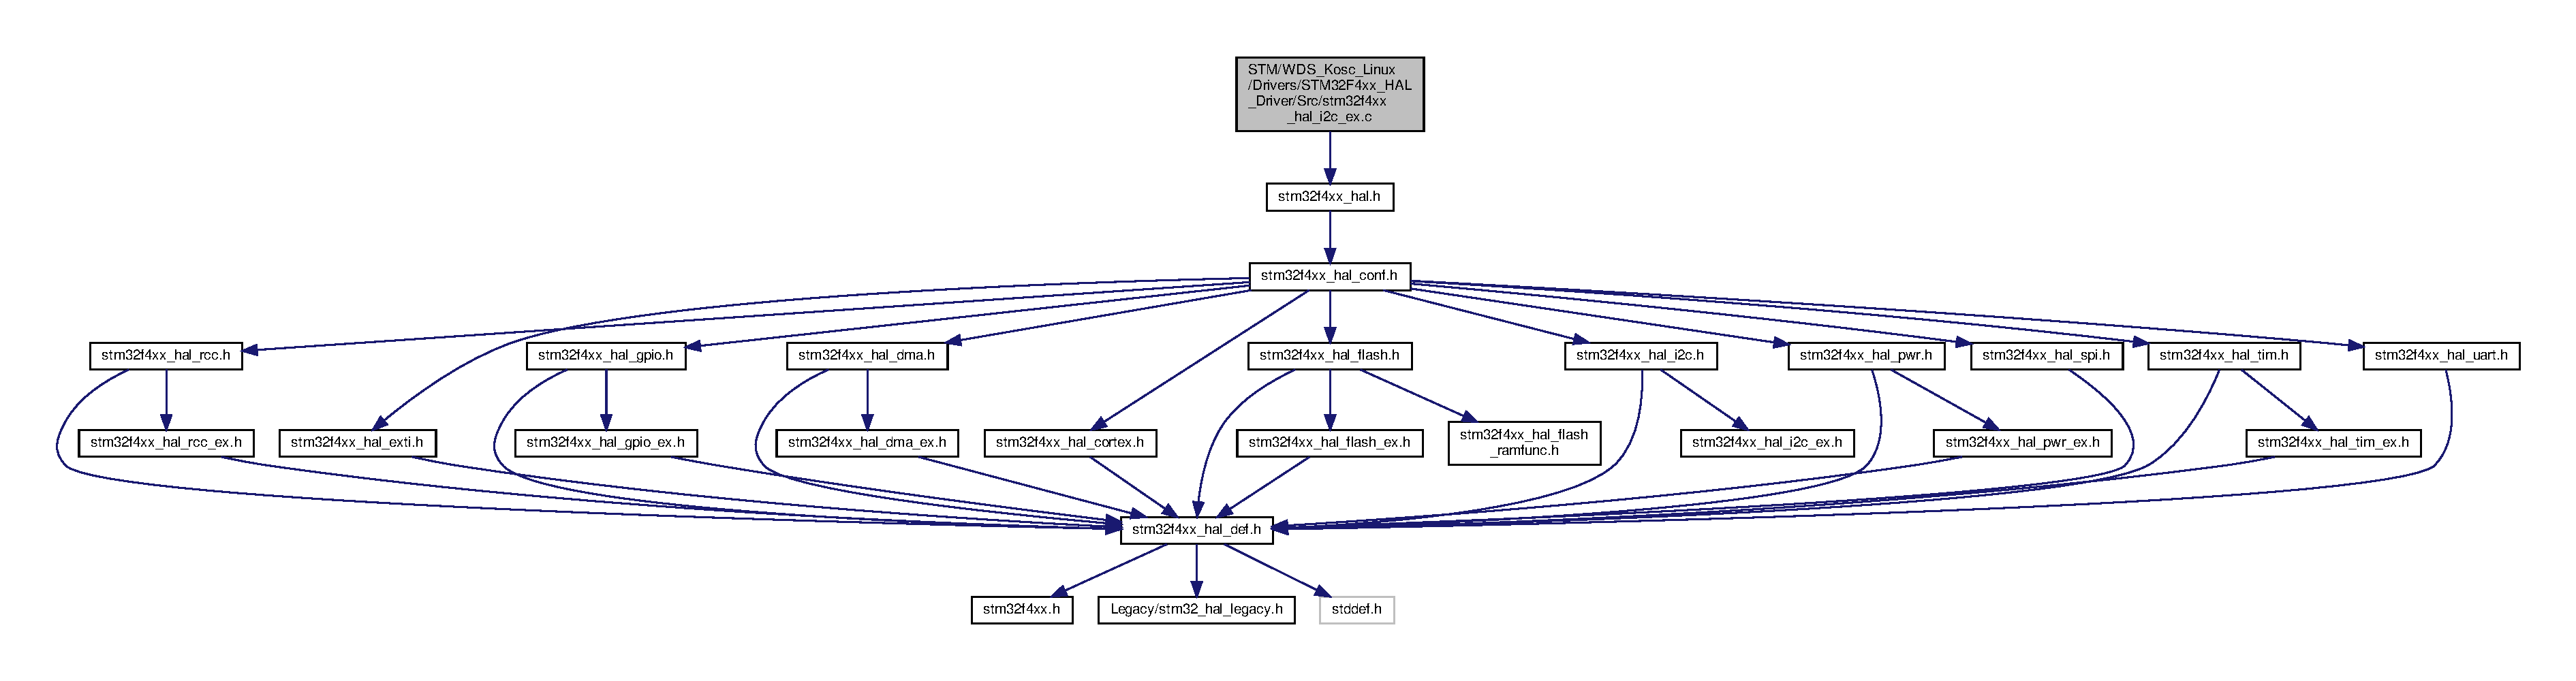
\includegraphics[width=350pt]{stm32f4xx__hal__i2c__ex_8c__incl}
\end{center}
\end{figure}


\subsection{Opis szczegółowy}
I2C Extension H\+AL module driver. This file provides firmware functions to manage the following functionalities of I2C extension peripheral\+: 

\begin{DoxyAuthor}{Autor}
M\+CD Application Team
\begin{DoxyItemize}
\item Extension features functions
\end{DoxyItemize}
\end{DoxyAuthor}
\begin{DoxyVerb}==============================================================================
             ##### I2C peripheral extension features  #####
==============================================================================

[..] Comparing to other previous devices, the I2C interface for STM32F427xx/437xx/
     429xx/439xx devices contains the following additional features :

     (+) Possibility to disable or enable Analog Noise Filter
     (+) Use of a configured Digital Noise Filter

                   ##### How to use this driver #####
==============================================================================
[..] This driver provides functions to configure Noise Filter
  (#) Configure I2C Analog noise filter using the function HAL_I2C_AnalogFilter_Config()
  (#) Configure I2C Digital noise filter using the function HAL_I2C_DigitalFilter_Config()\end{DoxyVerb}


\begin{DoxyAttention}{Uwaga}

\end{DoxyAttention}
\subsubsection*{\begin{center}\copyright{} Copyright (c) 2016 S\+T\+Microelectronics. All rights reserved.\end{center} }

This software component is licensed by ST under B\+SD 3-\/\+Clause license, the \char`\"{}\+License\char`\"{}; You may not use this file except in compliance with the License. You may obtain a copy of the License at\+: opensource.\+org/licenses/\+B\+S\+D-\/3-\/\+Clause 